%! Author = kyoto
%! Date = 11.09.2023

\vspace{3cm}
\tableofcontents

\newpage

\section{Описание предметной области.}
В сопровождении Элли и Малкольма, Грант обошел главное здание. Следом за ними шел мальчик. Грант любил детей. А как их
можно не любить, когда они так непосредственно, так страстно интересуются динозаврами. Гранту приходилось видеть, как в
музеях дети стояли с открытыми ртами, взирая на огромные скелеты, уходящие под самый потолок. Он часто спрашивал себя,
поче- му вымершие ящеры производят такое сильное впечатление на детей. Но потом он понял, что дети любят динозавров
потому, что эти гигантские создания воплощают в себе управляемую силу неограниченной власти. Динозавры символизируют
родителей, которых дети обожают, но боятся. Дети любят динозавров точно так же, как они любят своих родителей.

\section{Инфологическая модель.}
\begin{figure}[H]
	\centering
	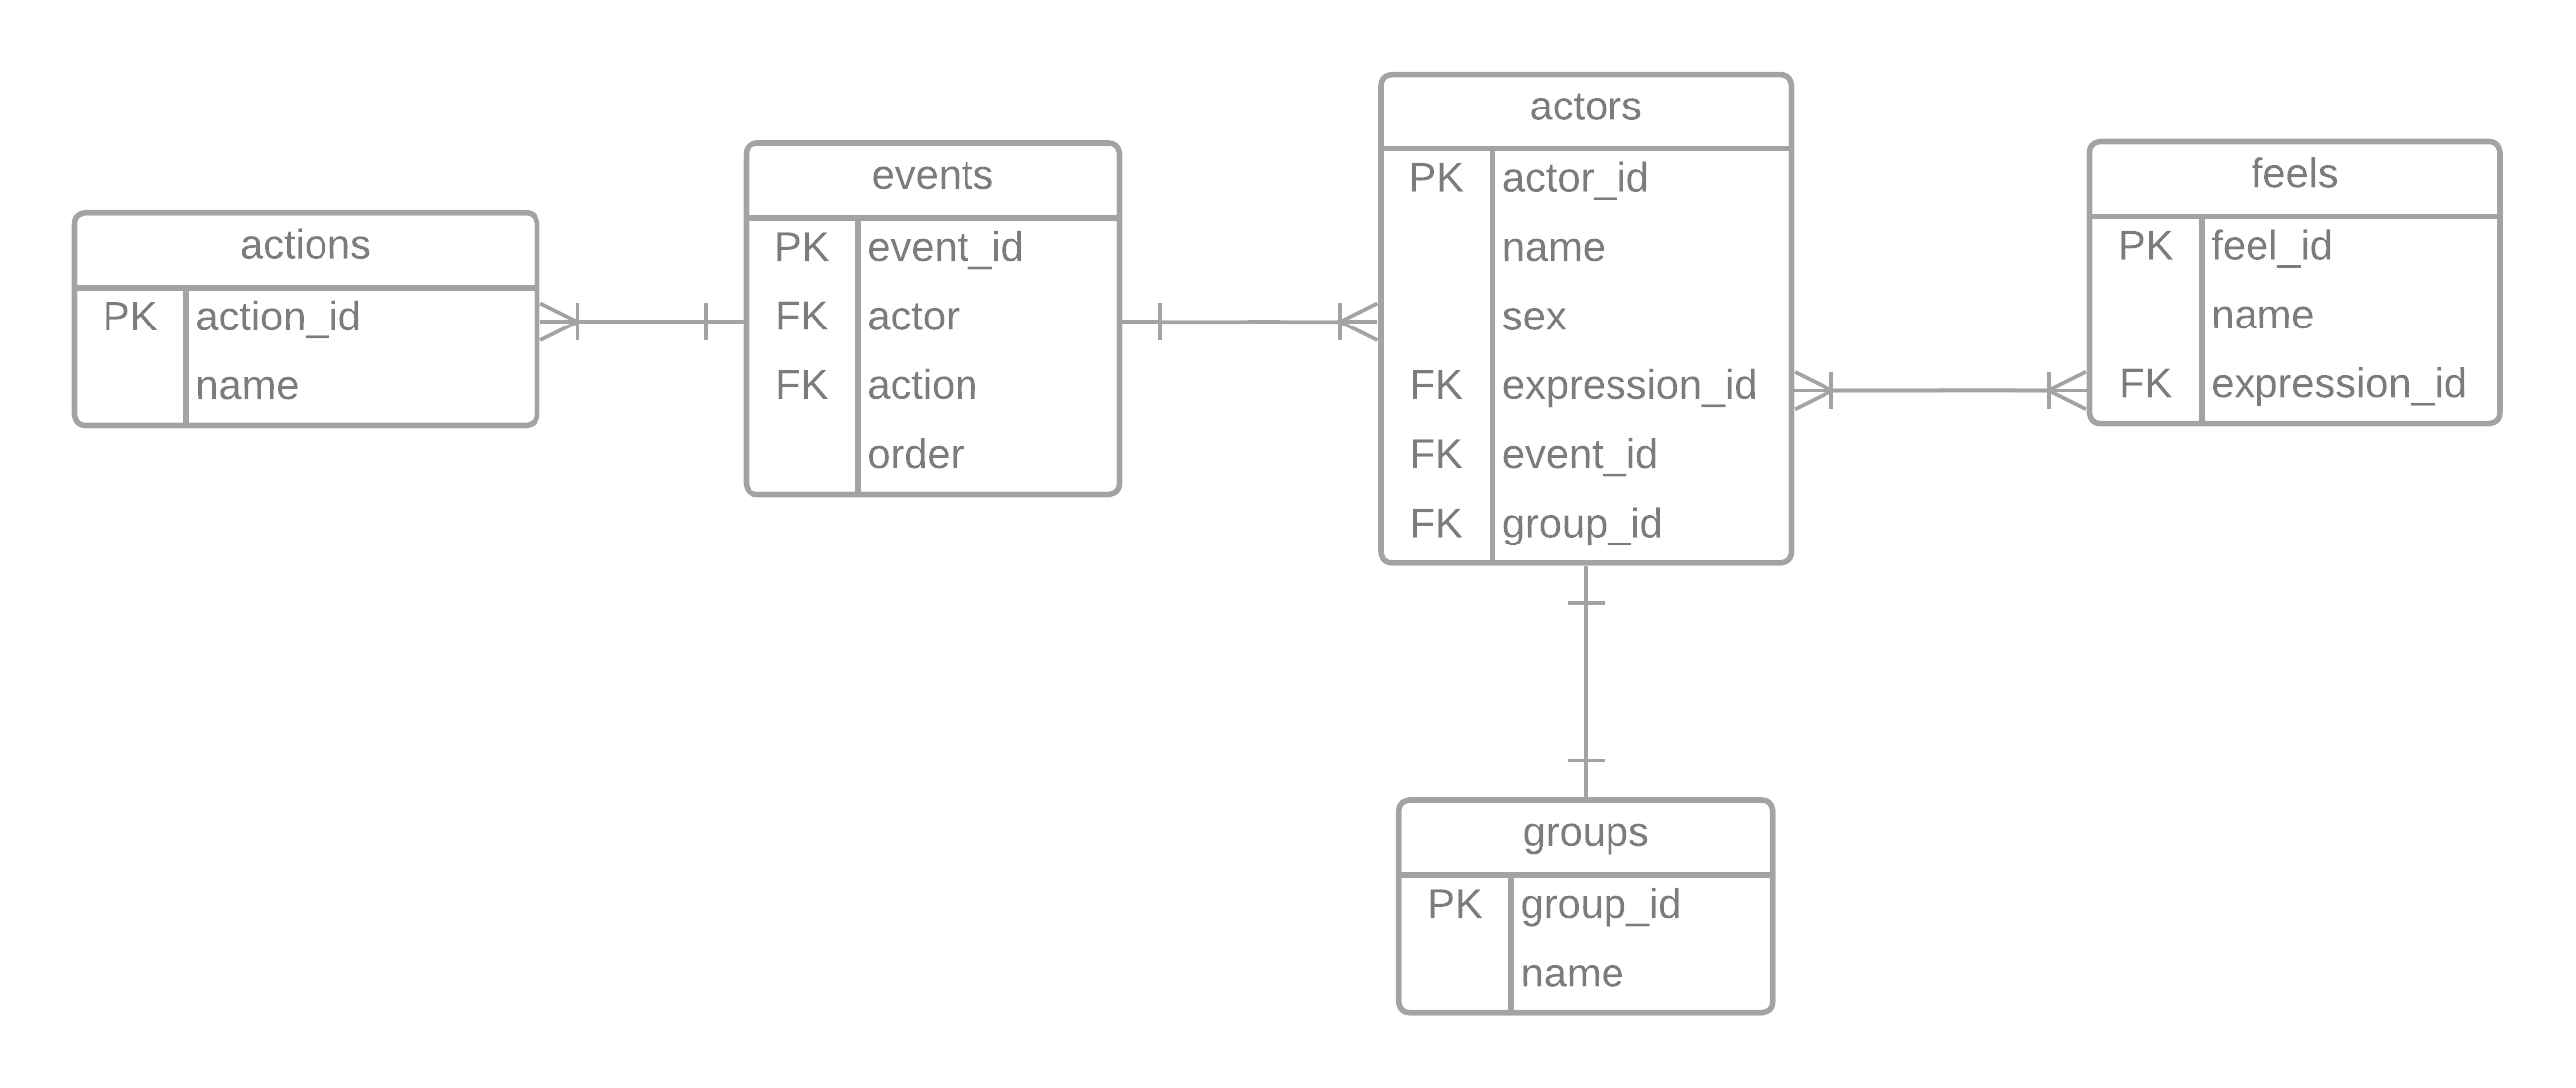
\includegraphics[scale=0.15]{img/info_model}
\end{figure}

\section{Даталогическая модель.}
\begin{figure}[H]
	\centering
	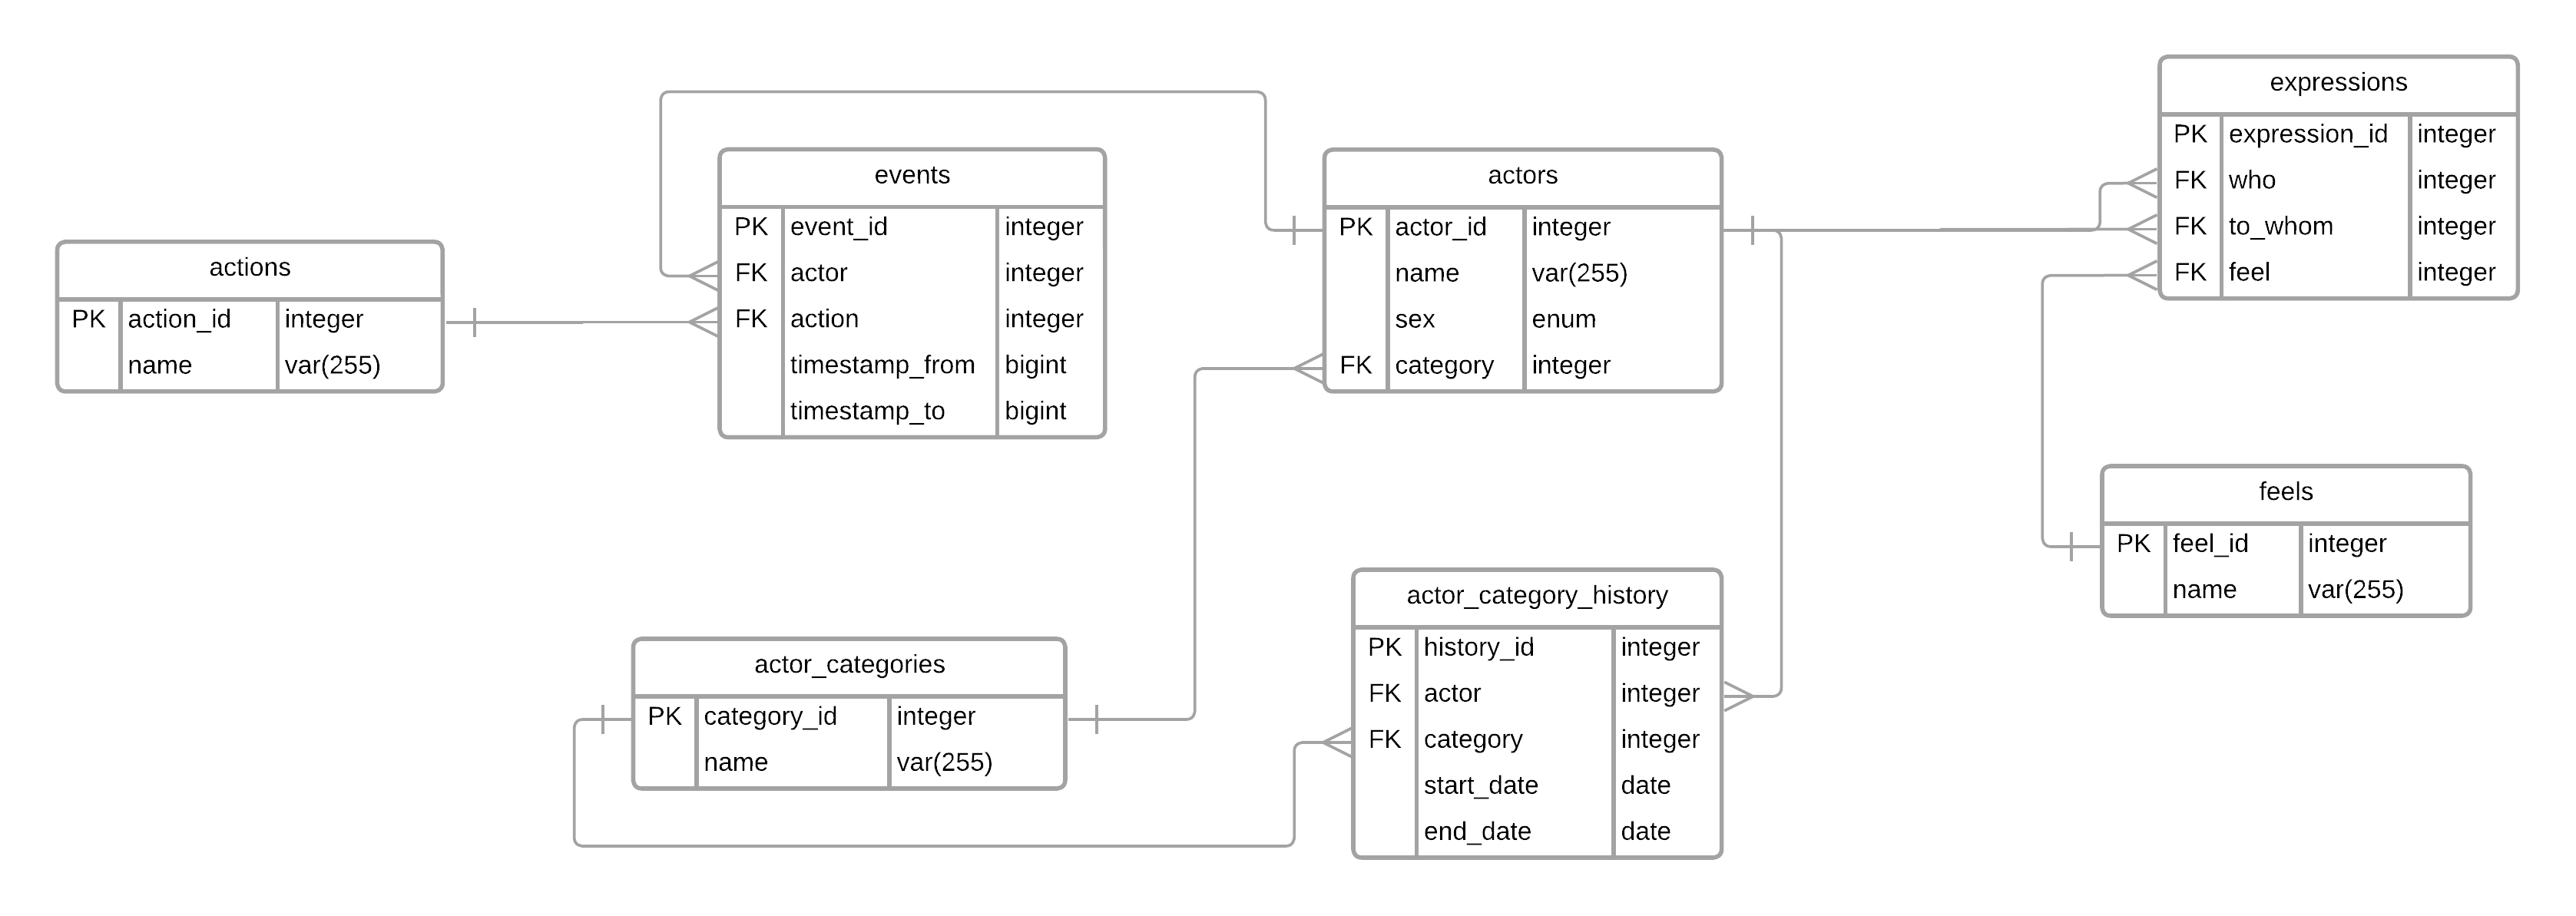
\includegraphics[scale=0.15]{img/data_model}
\end{figure}

\newpage

\section{Минимальное множество функциональных зависимостей.}
\begin{enumerate}
    \item actions
    \begin{itemize}
        \item action\_id -> name
    \end{itemize}
	\item feels
	\begin{itemize}
		\item feel\_id -> name
	\end{itemize}
	\item actor\_categories
	\begin{itemize}
		\item category\_id -> name
	\end{itemize}
	\item actors
	\begin{itemize}
		\item actor\_id -> name
		\item actor\_id -> sex
		\item actor\_id -> category
	\end{itemize}
	\item actor\_category\_history
	\begin{itemize}
		\item history\_id -> actor
		\item history\_id -> category
		\item history\_id -> start\_date
		\item history\_id -> end\_date
	\end{itemize}
	\item events
	\begin{itemize}
		\item event\_id -> actor
		\item event\_id -> action
		\item event\_id -> timestamp\_from
		\item event\_id -> timestamp\_to
	\end{itemize}
	\item expressions
	\begin{itemize}
		\item expression\_id -> who
		\item expression\_id -> to\_whom
		\item expression\_id -> feel
	\end{itemize}
\end{enumerate}

\section{Нормализация.}
\subsection{Первая нормальная форма.}
На пересечении столбца и строки всегда одно значение – условие нормализации выполняется.
\subsection{Вторая нормальная форма.}
Из-за того, что для каждой сущности первичный ключ состоит только из одного атрибута, для каждого атрибута реализована
полная функциональная зависимость – условие нормализации выполняется.
\subsection{Третья нормальная форма.}
Имя категории в actor\_categories зависит от category\_id, это создает транзитивную зависимость между actor\_id и name
в actor\_categories через category. Чтобы привести его к 3NF, нужно удалить таблицу actor\_categories, столбец category из actors и использовать
только связи в actor\_category\_history, при этом столбец category будет теперь не внешним ключом, а текстом, содержащим в себе имя категории.

После преобразования в 3NF функциональные зависимости остаются прежними, за исключением того, что в actors больше нет зависимости
actor\_id -> category

\subsection{BCNF.}
Для BCNF, для каждой нетривиальной функциональной зависимости X → Y, X должно быть потенциальным ключом. Все отношения
уже соответствуют BCNF, так как все левые части функциональных зависимостей являются ключами.

\section{Денормализация.}
Включение имени действия в events: Если часто требуется получать события вместе с именем действия, можно добавить поле name из таблицы actions в таблицу events.
Включение имени чувства в expressions: Если часто требуется получать выражения вместе с именем чувства, можно добавить поле name из таблицы feels в таблицу expressions.
Включение имени категории в actors: Если часто требуется получать категорию вместе с эктором, можно добавить поле name из таблицы actor\_categories в таблицу actors.
Эти денормализации могут улучшить производительность некоторых запросов, но могут также увеличить сложность обслуживания базы данных из-за дублирования данных.
Нужно внимательно рассмотреть потребности приложения перед принятием решения о денормализации.

\section{Заключение.}
В результате проведенной работы мы определили функциональные зависимости, привели схему базы данных к 3NF и BCNF. Мы также
рассмотрели возможные денормализации для оптимизации запросов. Теперь схема готова для эффективного использования в приложении,
с учетом требований к целостности данных и производительности.
